\section{Group Theory}
Here we list some group theory definitions and theorems used in the text. They are all attributed to \cite{group-theory-uon, armstrong_groups_1988} unless stated otherwise.

\subsection{Basic Definitions}
%\begin{definition}
%	A \textit{group} $G$ is a non-empty set with a binary operation $*$, such that
%	\begin{itemize}
%		\item For any $g, h \in G$, we have $g * h \in G$;
%		\item For any $g, h, k  \in G$, we have $(g * h) * k = g * (h * k)$;
%		\item There exists an identity element $e \in G$ such that for all $g \in G$, we have $e * g = g * e = g$;
%		\item For each $g \in G$, there exists an inverse element $g^{-1} \in G$ such that $g * g^{-1} = g^{-1} * g = e$. 
%	\end{itemize}
%\end{definition}

\begin{definition}
	A group $G$ is called \textit{abelian} if for any $g, h \in G$, we have that $g h = h g$. 
\end{definition}

\begin{definition}
	A \textit{subgroup} $H$ of a group $G$ is a subset of $G$ which is a group itself, denoted as $H \le G$. 
\end{definition}

\begin{definition}
	A \textit{normal subgroup} $N$ of a group $G$ is a subgroup of $G$ such that $gNg^{-1} = N$ for all $g \in G$. We denote $N \trianglelefteq G$. 
\end{definition}



\begin{definition}
	Given groups $N \trianglelefteq G$, $G / N = \{g N : g \in G\}$ is called the \textit{quotient group} of $N$, where the multiplication is defined by $g_1N g_2N = g_1g_2N$. 
\end{definition}

\begin{definition}
	Given groups $G$ and $H$, a group homomorphism $\phi: G \to H$ is a function such that $\phi(xy) = \phi(x) \phi(y)$ for any $x, y \in G$. It can be shown that $\phi(e) = e$ and $\phi(x^{-1}) = \phi(x) ^ {-1}$. The \textit{image} of $\phi$ is $\Img(\phi) = \{\phi(x) : x\in G\}$ and the \textit{kernel} of $\phi$ is $\Ker(\phi) = \{x \in G : \phi(x) = e\}$. It can be shown that $\Img(\phi) \le H$ and $\Ker(\phi) \trianglelefteq G$.  
\end{definition}

\begin{definition}
	Let $p$ be a prime. A \textit{$p$-group} is any group with order $p^k$ for $k \in \N$. Let $G$ be a group with order $p^k m$ and $\gcd\{p, m\} = 1$. Then any subgroup of order $p^k$ of $G$ is called a \textit{$p$-Sylow subgroup} of $G$. 
\end{definition}

\subsection{Symmetric Groups}
\begin{definition}  \label{def:permutation}
	Given a set $X$, a \textit{permutation} of $X$ is a bijection from $X$ to $X$. All the permutations of $X$ form a group under composition, which is the \textit{permutation group} of $X$, denoted by $S_X$. In particular, when $X = \{1, \dots, n\}$, we denote $S_X$ as $S_n$ and call it a \textit{symmetric group}. $S_n$ has order $n!$. 
\end{definition}

\begin{definition}
	A permutation that is a product of an even number of transpositions is called an \textit{even permutation}. The normal subgroup of $S_n$ consisting of all even permutations is the \textit{alternating group}, denoted as $A_n$. 
\end{definition}

We look at how symmetric groups can be generated by its elements. 

\begin{theorem} \label{thm:symmetric-12-12n}
	The transposition $(12)$ and $n$-cycle $(12 \dots n)$ together generate $S_n$ . 
\end{theorem}
\begin{proof}
	Consider the cyclic decomposition of each element in $S_n$, where each cyclic permutation can be written as 
	$
	(a_1a_2\dots a_k) = (a_1 a_k) \dots (a_1 a_3) (a_1 a_2). 
	$
	Note that $(ab) = (1a)(1b)(1a)$, therefore $(12), (13), \ldots (1n)$ together generate $S_n$. Also note that  
	$$(1k)=((k-1)k)\dots(34)(23)(12)(23)(34)\dots((k-1)k),$$
	therefore $(12), (23), \dots, ((n-1)n)$ together generate $S_n$. Finally note that 
	$$
	(k(k+1)) = (12\dots n)^{k-1} (12) (12\dots n)
	$$
	for $k = 2, 3, \dots n - 1$. Therefore $(12)$ and $(12 \dots n)$ together generate $S_n$. 
\end{proof}

The next two theorems are from \cite{generating-sets}. 

\begin{theorem} \label{thm:symmetric-ab-12n}
	For $1 \le a < b \le n$ such that $(b - a, n) = 1$, the transposition $(ab)$ and $n$-cycle $(12 \dots n)$ together generate $S_n$.
\end{theorem}
\begin{proof}
	Let $\sigma=(12 \ldots n)$, so $\sigma^i(a) \equiv a+i \bmod n$. Therefore $\sigma^{b-a}(a) \equiv b \bmod n$, and since $1 \le b \le n$, we have $\sigma^{b-a}(a)=b$. Since $(b-a, n)=1,\langle\sigma\rangle=\left\langle\sigma^{b-a}\right\rangle$ and $\sigma^{b-a}$ is an $n$-cycle sending $a$ to $b$, so $\sigma^{b-a}$ is of the form $(a b \ldots)$. Then
	$
	\langle(a b), \sigma\rangle=\left\langle(a b), \sigma^{b-a}\right\rangle=\langle(a b),(a b \ldots)\rangle .
	$
	Relabel the numbers $1,2 \ldots, n$ so that $(a b)$ turns into $(12)$ and $(a b \ldots)$ into $(12 \ldots n)$. Therefore $\langle(a b), \sigma\rangle=S_n$ by Theorem \ref{thm:symmetric-12-12n}.
\end{proof}

\begin{theorem} \label{thm:symmetric-prime}
	For a prime number $p$, any transposition and $p$-cycle together generate $S_p$.
\end{theorem}
\begin{proof}
	Relabel the numbers so that the $p$-cycle turns into $(12 \dots p)$. Suppose the transposition turns into $(ab)$, where $1 \le a < b \le n$. Since $p$ is prime and $1 \le b - a < p$, we have $(b - a, p) = 1$. The result thus follows from Theorem \ref{thm:symmetric-ab-12n}.
\end{proof}

\subsection{Isomorphism Theorems}

\begin{theorem}[First Isomorphism Theorem] \label{thm:first-iso}
	Suppose $\phi: G \to H$ is a group homomorphism. Then its kernel $\operatorname{Ker}(\phi)$ is a normal subgroup in $G$, its image $\operatorname{Im}(\phi)$ is a subgroup in $H$, and 
	$$
	G / \operatorname{Ker}(\phi) \cong \operatorname{Im}(\phi).
	$$
\end{theorem}

\begin{theorem}[Second Isomorphism Theorem] \label{thm:second-iso}
	Suppose $H \le G$ and $J \trianglelefteq G$. Then $HJ \le G$, $H \cap J \triangleleft H$ and $$
	(HJ) / J \cong H / (H \cap J). 
	$$
\end{theorem}
\begin{theorem}[Third Isomorphism Theorem] \label{thm:third-iso}
	Suppose $H, J \trianglelefteq G$ and $H \le J$. Then $J/H \trianglelefteq G/H$ and $$
	(G/H)/(J/H) \cong G / J.    $$
\end{theorem}



\subsection{Group Actions}



\begin{definition} \label{def:action}
	Given a group $G$ and a set $X$, if there is a homomorphism
	$$
	T: G \rightarrow S_X, \quad g \mapsto T_g,
	$$
	where $T_g(x) \in X$, then the group \textit{acts} on $X$ and $X$ is a $G$-set. 
\end{definition}

\begin{definition}
	For any $x \in X$, the $G$-orbit of $x$ in $X$ is
	$$\operatorname{Orb}_G(x) = \{ y = T_g(x) : g \in G \} \subseteq X.$$

	
%	\paragraph{Stabiliser} For any $x \in X$, the stabiliser of $x$ in $G$ is 
%	$$\Stab_G(x) = \{ g \in G : T_g(x) = x \} \le G. $$
%	It is a subgroup of $G$.
\end{definition}

\begin{definition} \label{def:transitive-action}
	Given a group $G$ acting on a set $X$, $G$ acts \textit{transitively} on $X$ if for any $x \in X$, $\Orb_G(x) = X$. Equivalently, for any $x, y\in X$, there exists $g \in G$, such that $T_g(x) = y$. 
\end{definition}

\begin{theorem}[Cauchy's Theorem] \label{thm:cauchy}
	Let $p$ be a prime number. Let $G$ be a finite group such that $p$ divides the order of $G$. Then $G$ contains an element of order $p$. 
\end{theorem}

\subsection{Solvable Groups}

The following is a restatement and proof of Theorem \ref{thm:soluble-main}, based on \cite{Stewart}.

\begin{theorem} \label{thm:soluble-main-appendix}
	Let $G$ be a group, $H \le G$ and $N \trianglelefteq G$. Then 
	\begin{enumerate}
		\item If $G$ is solvable, then $H$ is solvable;
		\item If $G$ is solvable, then $G / N$ is solvable; 
		\item If $N$ and $G / N$ are solvable, then $G$ is solvable. 
	\end{enumerate}
\end{theorem}
\begin{proof}
	\begin{enumerate}
		\item If $G$ is solvable, then there exists a finite series of subgroups $G_i$ of $G$ for $i = 0, 1, \dots, n$ satisfying Definition \ref{def:soluble}. Let $H_i = G_i \cap H$. Then $H$ has a series of subgroups $H_i$ such that $\{ e \} = H_0 \triangleleft H_1 \triangleleft \dots \triangleleft H_n = H.$
		For each $i = 0, 1, \dots, n - 1$, 
		$$
		\frac{H_{i+1}}{H_i} 
		= \frac{G_{i+1} \cap H}{G_i \cap (G_{i+1} \cap H)}
		\cong \frac{G_i(G_{i+1} \cap H)} {G_i}
		$$
		by Theorem \ref{thm:second-iso}, and ${G_i(G_{i+1} \cap H)}/{G_i}$ is a subgroup of the abelian group $G_{i+1} / G_{i}$. Hence $H_{i+1} / H_{i}$ is abelian and $H$ is solvable.
		\item Take $G_i$ as before. Then $G / N$ has a series
		$N/N = G_0 N / N \triangleleft G_1 N / N \triangleleft \dots \triangleleft G_n N / N  =  G / N. $
		For each $i = 0, 1, \dots, n - 1$, 
		$(G_{i+1} N / N) / (G_{i} N / N) \cong (G_{i+1} N) / (G_i N)$
		by Theorem \ref{thm:third-iso}. Then 
		$$
		\frac{G_{i+1} N}{G_i N} =\frac{G_{i+1}\left(G_i N\right)}{G_i N} \cong \frac{G_{i+1}}{G_{i+1} \cap\left(G_i N\right)} \cong \frac{G_{i+1} / G_i}{\left(G_{i+1} \cap\left(G_i N\right)\right) / G_i},
		$$
		which is a quotient of the abelian group $G_{i+1} / G_i$, so is abelian. Hence $G / N$ is solvable.
		\item There exist two series
		$$
		\begin{aligned}
			\{ e \} & =N_0 \triangleleft N_1 \triangleleft \ldots \triangleleft N_r=N, \\
			N / N & =G_0 / N \triangleleft G_1 / N \triangleleft \ldots \triangleleft G_s / N=G / N
		\end{aligned}
		$$
		with $N_{i+1} / N_{i}$ abelian for each $i = 0, 1, \dots, r-1$ and $(G_{i+1} / N)  / (G_{i} / N) \cong G_{i+1} / G_i $ abelian for each $i = 0,1, \dots, s-1$. Combining them gives the series of subgroups of $G$:
		$$
		\{ e \}=N_0 \triangleleft N_1 \triangleleft \ldots \triangleleft N_r=N=G_0 \triangleleft G_1 \triangleleft \ldots \triangleleft G_s=G .
		$$
		The quotients are either $N_{i+1} / N_i$  or $G_{i+1} / G_i$ and are all abelian. Therefore $G$ is solvable.
	\end{enumerate}
\end{proof}
in Example \ref{exm:correspondence}

\section{Solvability by Radicals} \label{sec:radical-alter}

We now establish (one direction of) the Galois' Theorem using an alternative method based on \cite{Stewart}. This proof addresses the potential problem in the proof of Theorem \ref{thm:galois-theorem} that the radical extension might not be exactly the splitting field but contains it.  

The proof for the following theorem is original. 
\begin{theorem} \label{thm:fix-extension-normal}
	Let $L$ be a field and let $G \le \Aut(L)$ be finite. Let $K = \Fix(G)$. Then $L/K$ is a normal extension.
\end{theorem}

\begin{proof}
	
	Let $f$ be an irreducible polynomial over $K$ with a root $\alpha \in L$. Consider the finite set $S = \Orb_G(\alpha) = \{ \alpha_1, \ldots, \alpha_n\} \subseteq L$. Let $h(t) = \prod_{i = 1} ^n (t - \alpha_i)$, which splits in $L$.
	
	Note that each $\sigma \in G$ maps $S$ to itself. Therefore, $h$ is fixed by $G$, and all of its coefficients are in $\Fix(G) = K$. We then claim that $h$ is irreducible over $K$. Suppose that $h$ is reducible over $K$, then $\Gal(h)$ does not act transitively on $S$ by Theorem \ref{thm:galois-action-transitive-irreducible}. Let $\Sigma = K(\alpha_1, \dots, \alpha_n)$ be the splitting field of $h$ contained in $L$.  Any $\sigma \in G$ is a $K$-automorphism of $L$ which permutes $\alpha_i$, and thus for any $\gamma \in \Sigma$, we have $\sigma(\gamma) \in \Sigma$ (using a similar argument as in the proof of Theorem \ref{thm:galois-group-determined-by-generator}). Thus $\sigma | _ \Sigma \in \Gal(h)$. 
	Then each element in $G$ defines an element in $\Gal(h)$ and $G$ acts transitively on $S$ by construction, and thus we have a contradiction. 
	
	Since $\alpha$ is a root of $h$ and $h$ is irreducible over $K$, $h$ is the minimal polynomial of $\alpha$ over $K$. Thus $h = f$ and $f$ splits in $L$. Thus the extension $L/K$ is normal. 
\end{proof}


\begin{theorem} \label{thm:radical-3}
	If $K$ is a subfield of $\mathbb{C}$ and $L / K$ is normal and radical, then $\Gal(L / K)$ is solvable.
\end{theorem}

\begin{proof}
	Let $L=K\left(\alpha_1, \ldots, \alpha_n\right)$ with $\alpha_j^{n_j} \in K\left(\alpha_1, \ldots, \alpha_{j-1}\right)$. By Theorem \ref{thm:radical-all-prime}, we may assume that $n_j$ is prime for all $j$. We prove the result by induction on $n$. 
	% In particular there is a prime $p$ such that $\alpha_1^p \in K$.
	
	If $n = 0$, we have $L = K$, and the case is trivial.
	If $n \ge 1$ and $\alpha_1 \in K$, then $L=K\left(\alpha_2, \ldots, \alpha_n\right)$ and $\Gal(L / K)$ is solvable by induction.
	Let $n \ge 1$ and $\alpha_1 \notin K$. Let $p = n_1$, which is prime, and then $\alpha_1^p \in K$.  Then $L$ contains a primitive $p$-th root of unity $\omega$ by the proof of Theorem \ref{thm:radical-simple-solvable}. Let $M = K(\omega)$ and let $N = M(\alpha_1)$. Consider the chain of subfields $K \subseteq M \subseteq N \subseteq L$. We now prove the solvability of $\Gal(L/N), \Gal(N/M), \Gal(L/M), \Gal(M/K)$, and $\Gal(L/K)$ step by step:
	
	\begin{itemize}
		\item Since $L=N\left(\alpha_2, \ldots, \alpha_n\right)$, $L / N$ is a normal radical extension. By induction $\Gal\left(L / N\right)$ is solvable. 
		\item Since $ \omega \in M$ and $\alpha_1^p \in M$, the proof of Theorem \ref{thm:radical-2} implies that $N$ is a splitting field for $t^p-\alpha_1^p$ over $M$. Thus $N / M$ is normal. By Theorem \ref{thm:radical-2}, $\Gal\left(N / M\right)$ is abelian and hence solvable. 
		\item  $L/ K$ is finite and normal, and so is $L / M$. Apply Theorem \ref{thm:correspondence-quotient} to $L / M$ to deduce that
		$
		\Gal\left( N / M \right) \cong \Gal(L / M) / \Gal\left(L / N\right).
		$
		Hence by Theorem \ref{thm:soluble-main},  $ \Gal(L / M)$ is solvable.
		\item Clearly $M$ is the splitting field for $t^p-1$ over $K$. Then the extension $M / K$ is normal. By Theorem \ref{thm:radical-1}, $\Gal(M / K)$ is abelian and hence solvable.
		\item  Apply Theorem \ref{thm:correspondence-quotient} to $L / K$ to obtain
		$
		\Gal(M / K) \cong \Gal(L / K) / \Gal(L / M). 
		$
		Theorem \ref{thm:soluble-main} shows that $\Gal(L / K)$ is solvable, completing the induction step.
	\end{itemize}
\end{proof}


\begin{definition}
	A \textit{normal closure} of a field extension $L / K$ is an extension $N$ of $L$ such that  $N / K$ is normal and if $L \subseteq M \subseteq N$ and $M / K$ is normal, then $M = N$.
\end{definition}

\begin{theorem} \label{thm:radical-closure}
	If $L / K$ is a radical extension in $\mathbb{C}$ and $N$ is the normal closure of $L / K$, then $N / K$ is radical.
\end{theorem}

\begin{proof}
	Let $L=K\left(\alpha_1, \ldots, \alpha_m\right)$ with $\alpha_i^{n_i} \in K\left(\alpha_1, \ldots, \alpha_{i-1}\right)$. Let $f_i = \mu _ {\alpha_i}$ over $K$. Then the splitting field of $f = \prod_{i=1}^m f_i$ is $N$. For every root $\beta_{i j}$ of $f$,  Theorem \ref{thm:automorphism-from-zeros} implies the existence of a $K$-automorphism $\tau$ of $N$ such that $\tau(\alpha_i) = \beta_{ij}$. Thus combining $\beta_{ij}$ gives a radical sequence for $N$.
\end{proof}





\begin{theorem}[Galois' Theorem] \label{thm:radical-galois-soluble}
	Let $f$ be a polynomial over a subfield $K$ of $\mathbb{C}$. If $f$ is solvable by radicals, then $\Gal(f)$ is solvable.
\end{theorem}

\begin{proof}
	Let $F$ be the splitting field of $f$ over $K$. We have $K \subseteq F \subseteq M$ where $M / K$ is a radical extension. Let $K_0 = \Fix(\Gal(F / K))$, and let $N$ be the normal closure of $M / K_0$. Then
	$
	K \subseteq K_0 \subseteq F \subseteq M \subseteq N.
	$
	Since $M / K_0$ is radical, Theorem \ref{thm:radical-closure} implies that $N / K_0$ is a normal radical extension. By Theorem \ref{thm:radical-3}, $\Gal\left(N / K_0\right)$ is solvable.
	By Theorem \ref{thm:fix-extension-normal}, the extension $F / K_0$ is normal. By Theorem \ref{thm:correspondence-quotient}
	$
	\Gal\left(F / K_0\right) \cong \Gal\left(N / K_0\right) / \Gal(N / F).
	$
	Theorem \ref{thm:soluble-main} implies that $\Gal\left(F / K_0\right)$ is solvable. But $\Gal(F / K)=\Gal\left(F / K_0\right)$, so $\Gal(F / K)$ is solvable.
\end{proof}


\section{Ruler-and-Compass Constructions}
We first prove a lemma to help us show that $\pi$ cannot be rational.

\begin{lemma}\label{lemma:pre-pi-irrational-lemma}
    Let $f:\Z \rightarrow \Z$ be a function such that $f(n)\rightarrow 0$ as $n \rightarrow \infty$. Then $\exists N \in \Z$ with $f(n)=0 \forall n\geq N$.
\end{lemma}

\begin{proof}
    By definition our function $f(n) \rightarrow 0$ as $n \rightarrow \infty$, so we can say that there must be an integer $N$ such that $|f(n)-0|<0.5$ for $n\geq N$. Since, $f(n) \in \Z$ this means that $f(n)=0; \forall n \geq N$.
\end{proof}

\begin{theorem}
    $\pi$ is not rational.
\end{theorem}

\begin{proof}

    Consider the following integral:

    $$I_n = \int_{-1}^{1} (1-x^2)^n \cos(\alpha x)dx. $$

    By integration by parts twice, we obtain:
    $\alpha^2I_n=2n(2n-1)I_{n-1}-4n(n-1)I_{n-2}$ for $n\geq 2$.

    Then by induction it is possible to show that $\alpha^{2n+1}I_n=n!(P_n \sin(\alpha)+Q_n \cos(\alpha))$.
    Here $P_n$ and $Q_n$ are polynomials in $\alpha$ of degree less than $2n+1$.

    Now assume towards a contradiction that $\pi = \frac{a}{b}$ where $a,b\in \Z$. By substituting $\alpha = \pi/2$ into equation above, we see that $\frac{\alpha^{2n+1}}{n!}$ must be an integer. So let $J_n = \frac{\alpha^{2n+1}}{n!}$, and by the definition of $I_n$ we get $J_n = \frac{\alpha^{2n+1}}{n!}\cdot \int_{-1}^{1} (1-x^2)^n \cos(\frac{\pi}{2} x)dx$.

    Since the integrand is greater than zero in our range, this means that $J_n \neq 0 \forall n \in \N$. Now by considering $|J_n|$, we see that $|J_n| \leq \frac{|\alpha|^{2n+1}}{n!} \cdot \int_{-1}^1 \cos(\frac{\pi}{2}x)dx \leq 2\frac{|\alpha|^{2n+1}}{n!}$. Thus as $n\rightarrow \infty$, we have that $J_n\rightarrow 0$. However, this contradicts Lemma \ref{lemma:pre-pi-irrational-lemma}, as $J_n$ must be an integer, so our assumption must be wrong and hence $\pi$ cannot be rational.
\end{proof}

\section{Figures}



\begin{figure}[p]
	\centering
	\begin{tikzpicture}
		\draw[->, densely dotted] (-2.5,0) -- (2.5,0) node[below] {$\Re z$};
		\draw[->, densely dotted] (0,-2.5) -- (0,2.5) node[right] {$\Im z$};
		%		\draw[densely dotted] (0, 0) circle (1); 
		%		\draw[densely dotted] (0, 0) circle (1.26); 
		
		\fill (1.26, 0) circle (2pt) node[right] {$\sqrt[3]{2}$};
		\fill (-0.63, 1.09) circle (2pt) node[above] {$\zeta \sqrt[3]{2}$};
		\fill (-0.63, -1.09) circle (2pt) node[below] {$\zeta^2 \sqrt[3]{2}$};
		%		\fill (1, 0) circle (1pt) node[left] {$1$};
		%		\fill (-0.5, -0.866) circle (2pt) node[above] {$\zeta^ 2$};
		%		\fill (-0.5, 0.866) circle (2pt) node[below] {$\zeta$};
		\draw[->-=0.4, red] (1.26, 0) arc   (0:120:1.26)  node[midway] {$\tau$};
		\draw[->-=0.4, red] (-0.63, 1.09) arc (120:240:1.26)  node[midway] {$\tau$};
		\draw[->-=0.4, red] (-0.63, -1.09) arc (240:360:1.26) node[midway] {$\tau$};
		\draw[->-=0.5, blue] (-0.63, -1.09) to [out=120,in=240] node[right] {$\rho$} (-0.63, 1.09); 
		\draw[->-=0.5, blue] (-0.63, 1.09) to [out=300,in=60] node[right] {$\rho$} (-0.63, -1.09); 
		
		
		
		%		\draw[very thin,color=gray] (-3,-3) grid (3,3);
	\end{tikzpicture}
	\caption{Actions of $\tau$ and $\rho$ on the roots of $f(t) = t^3 - 2$ in Example \ref{exm:correspondence}.}
	\label{fig:example-action}
		\end{figure}
	\begin{figure}[p]
		
	\centering
	\begin{tikzpicture}
		
		\node(A1) 										{\textcolor{blue}{$\Q(\zeta, \sqrt[3]{2})$}};
		\node(B1) [below left=2cm and 2cm of A1]      	{\textcolor{red}{$\Q(\zeta)$}}; 
		\node(B2) [below left=1cm and -0.7cm of A1]     {\textcolor{brown}{$\Q(\sqrt[3]{2})$}}; 
		\node(B3) [right=0.7cm of B2]					{\textcolor{orange}{$\Q(\zeta \sqrt[3]{2} )$}}; 
		\node(B4) [right=0.7cm of B3]					{\textcolor{purple}{$\Q(\zeta^2 \sqrt[3]{2} )$}}; 
		\node(C1) [below=3cm of A1]						{$\Q$}; 
		
		\draw[thick](A1) -- node[left]{3} (B1); 
		\draw[thick](A1) -- node[right]{2} (B2); 
		\draw[thick](A1) -- node[right]{2} (B3); 
		\draw[thick](A1) -- node[right]{2} (B4); 
		
		\draw[thick](C1) -- node[left]{2} (B1); 
		\draw(C1) -- node[left]{3} (B2); 
		\draw(C1) -- node[left]{3} (B3); 
		\draw(C1) -- node[left]{3} (B4); 
		
	\end{tikzpicture}
	\caption{Lattice diagram for intermediate fields of $\Q(\zeta, \sqrt[3]{2})$, where $\zeta = e^{2\pi i / 3}$ in Example \ref{exm:correspondence}. Each line from a lower field $K$ to an upper field $L$ indicates a field extension $L/K$. The number on each line indicates the degree of $L/K$, i.e. $[L:K]$. A thick line indicates that $L/K$ is a normal (and Galois) extension. }
	\label{fig:example-intermidate-fields}
		\end{figure}
\begin{figure}[p]
	\centering
	\begin{tikzpicture}
		\node(A1) 										{\textcolor{blue}{$\langle e \rangle$}};
		\node(B1) [above left=2cm and 2cm of A1]      	{\textcolor{red}{$\langle \tau \rangle$}}; 
		\node(B2) [above left=1cm and -0.7cm of A1]     {\textcolor{brown}{$\langle \rho \rangle$}}; 
		\node(B3) [right=0.7cm of B2]					{\textcolor{orange}{$\langle \tau \rho  \rangle$}}; 
		\node(B4) [right=0.7cm of B3]					{\textcolor{purple}{$\langle \tau ^ 2 \rho  \rangle$}}; 
		\node(C1) [above=3cm of A1]						{$G$}; 
		
		\draw[thick](A1) -- node[left]{3} (B1); 
		\draw[thick](A1) -- node[right]{2} (B2); 
		\draw[thick](A1) -- node[right]{2} (B3); 
		\draw[thick](A1) -- node[right]{2} (B4); 
		
		\draw[thick](C1) -- node[left]{2} (B1); 
		\draw(C1) -- node[left]{3} (B2); 
		\draw(C1) -- node[left]{3} (B3); 
		\draw(C1) -- node[left]{3} (B4); 
	\end{tikzpicture}
	\caption{Lattice diagram for subgroups of $G = \Gal(t^3 - 2)$ in Example \ref{exm:correspondence}. Each line from a lower group $H$ to an upper group $G$ indicates that $H$ is a subgroup of $G$. The number on each line indicates the index of $H$ in $G$, i.e. $[G:H]$. A thick line indicates that $H$ is a normal subgroup of $G$. }
	 \label{fig:example-subgroups}
\end{figure}

\begin{figure}[p]
	\centering
	\begin{tikzpicture}
		\node(K) {$K$};
		\node(L) [above=1.3cm of K] {$L$}; 
		\node(M) [right=2cm of K] {$M$};
		\node(N) [above=1.3cm of M] {$N$}; 
		
		\draw[->] (K) --  node[below] {$t^p - c$} (M);
		\draw[->] (L) --  node[above] {$t^p - c$} (N);
		\draw[->] (K) --  node[left] {$f(t)$} (L);
		\draw[->] (M) --  node[right] {$f(t)$} (N);
		\draw[->] (K) --  node[above] {$f(t)(t^p - c)$} (N);
	\end{tikzpicture}
	\caption{Field extensions in the proof of Theorem \ref{thm:solvable:chain}. For example, an arrow from field $K$ to field $L$ with label $f(t)$ indicates that $L$ is the splitting field of $f(t)$ over $K$. }
	\label{fig:solvable-chain}
\end{figure}

\begin{figure}[p]
	\centering
	\begin{tikzpicture}
		\node(Q) {$\Q$}; 
		\node(A) [above=1.4cm of Q] {$\mathbb A$}; 
		\node(C) [above=1.2cm of A] {$\mathbb C$}; 
		
		
		\node(Rad) [above left=0.7cm and 1cm of Q] {numbers expressible by radicals}; 
		
		\draw (Q) -- node[left]{radical extensions} (Rad);
		\draw (Rad) --  node[above] {$\subsetneqq$}(A); 
		\draw (Q) -- node{algebraic closure} (A); 
		\draw (A) -- (C); 
		
		\node(R) [above right=0.2 and 4cm of A] {$\R$}; 
		\draw(A) -- node {transcendental numbers} (R); 
		\draw(R) -- node[above] {algebraic closure} (C); 
		\draw(Q) -- node[right] {irrational numbers} (R); 
	\end{tikzpicture}
	\caption{Hasse diagram for $\Q, \mathbb A, \R, \C$ and numbers expressible by radicals \cite{visual-algebra}. }
	\label{fig:hasse}
\end{figure}



%\FloatBarrier
\begin{figure}[p]
	\centering
	\scalebox{0.7}{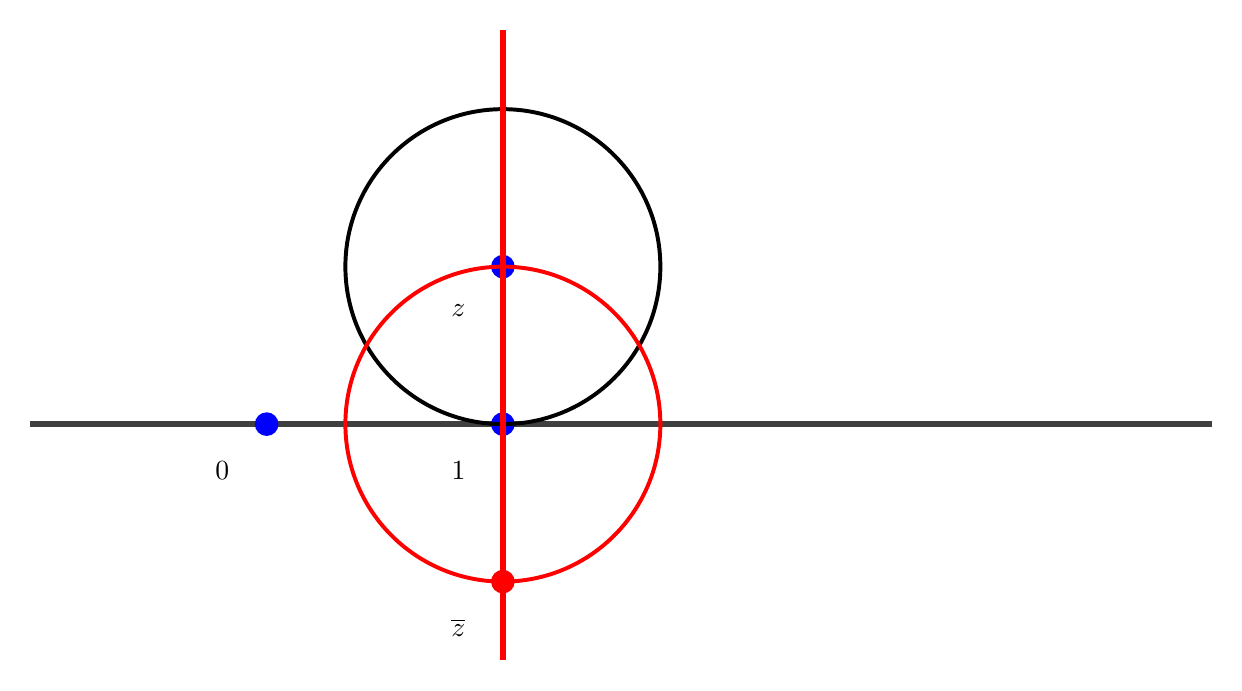
\begin{tikzpicture}
			\draw[line width = 0.7mm, darkgray] (0,0) -- (15,0);
			\fill[blue] (3,0) circle (0.15cm);
			\fill[blue] (6,0) circle (0.15cm);
			\fill[blue] (6,2) circle (0.15cm);
			\node[below left=10pt] at (3,0) {$0$};
			\node[below left=10pt] at (6,0) {$1$};
			\node[below left=10pt] at (6,2) {$z$};
			\draw[color=black, line width = 0.5mm] (6,2) circle [radius=2];
			\draw[line width = 0.7mm, red] (6,-3) -- (6,5);
			\draw[color=red, line width = 0.5mm] (6,0) circle [radius=2];
			\fill[red] (6,-2) circle (0.15cm);
			\node[below left=10pt] at (6,-2) {$\overline{z}$};
	\end{tikzpicture}}
	\caption{Example of case one of the proof of Lemma \ref{lemma:conjugate-in-Pn}.}
	\label{fig:case-1-conjugate}
\end{figure}
%\FloatBarrier



%\FloatBarrier
\begin{figure}[p]
	\centering
	\scalebox{0.7}{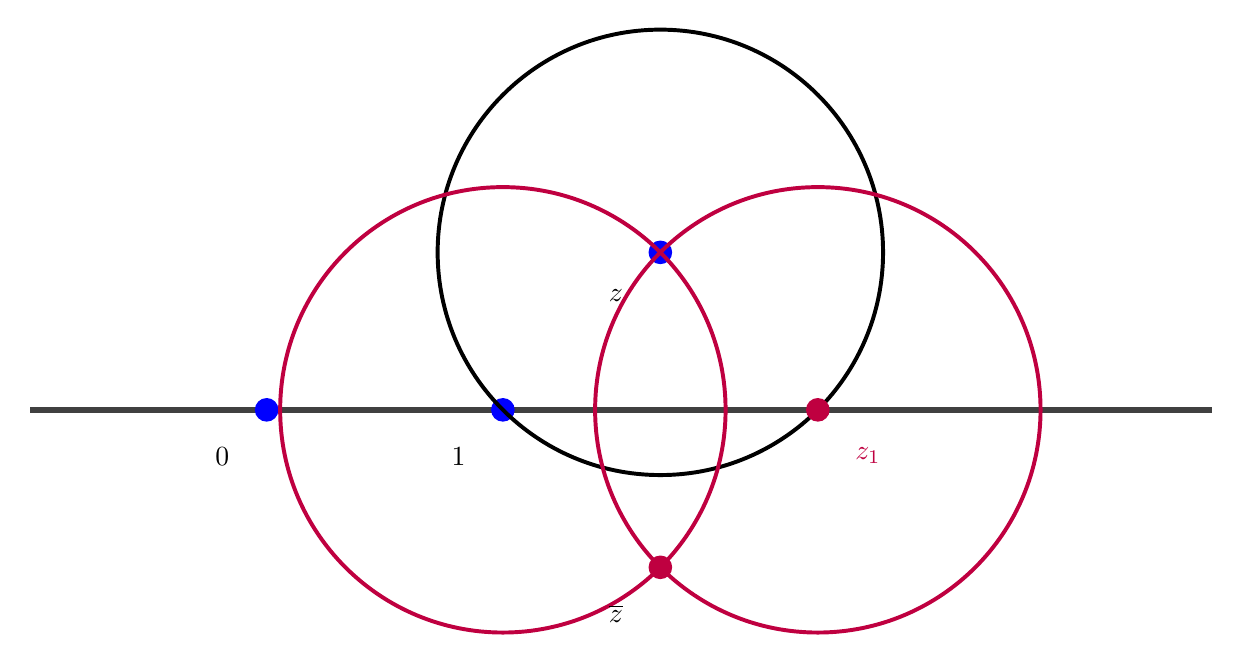
\begin{tikzpicture}
			\draw[line width = 0.7mm, darkgray] (0,0) -- (15,0);
			\fill[blue] (3,0) circle (0.15cm);
			\fill[blue] (6,0) circle (0.15cm);
			\node[below left=10pt] at (3,0) {$0$};
			\node[below left=10pt] at (6,0) {$1$};
			\fill[blue] (8,2) circle (0.15cm);
			\node[below left=10pt] at (8,2) {$z$};
			\draw[color=black, line width = 0.5mm] (8,2) circle [radius=2.828427];
			\fill[purple] (10,0) circle (0.15cm);
			\node[below right=10pt, color = purple] at (10,0) {$z_1$};
			\draw[color=purple, line width = 0.5mm] (10,0) circle [radius=2.828427];
			\draw[color=purple, line width = 0.5mm] (6,0) circle [radius=2.828427];
			\fill[purple] (8,-2) circle (0.15cm);
			\node[below left=10pt] at (8,-2) {$\overline{z}$};
	\end{tikzpicture}}
	\caption{Example of case two of the proof of Lemma \ref{lemma:conjugate-in-Pn}.}
	\label{fig:case-2-conjugate}
\end{figure}
%\FloatBarrier

		


